% falar sobre o que é uma transformada integral.
% Exemplo e definiçã 
A transformada de Laplace é uma transformada integral que associa funções $\mathbb{R} \mapsto \mathbb{C}$.
É usada para modelar sistemas em que há mudanças rápidas de comportamentos (a.k.a ``impulsos''). Em
geral comportamentos que saem de um regime homogêneo em um instante $t$.

\begin{theorem}
  Definição: No espaço das funções $\mathcal{F}$ temos funções do tipo $f:\mathbb{R}_{+} \mapsto \mathbb{C}$,
  definimos a transformada de laplace como
  \begin{equation}
  F(s) \equiv \mathcal{L} \{ f \} (s) = \int_{-\infty}^{\infty} e^{-st} f(t) dt
  \label{eq:transformada_laplace}
  \end{equation}
\end{theorem}

\begin{figure}[h!]
  \centering
  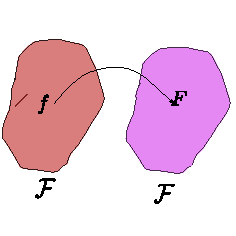
\includegraphics[width=0.6\textwidth]{./images/transformada_laplace.pdf}
\end{figure}


% Define the functions
\def\fx{exp(\x) / (\x + 1)}
\def\gx{(\x + 2) / (\x - 1)}
\def\hx{(\x - 4) / (\x + 3) + \x / 2 + 2}
\begin{figure}
  \centering
\begin{tikzpicture}
  % Axis
  \draw[->] (0,0) -- (7,0) node[right] {$x$};
  \draw[->] (0,-1) -- (0,7) node[above] {$y$};

  % Plot f(x) for 0 <= x <= 2
  \draw[domain=0:2, samples=100, smooth, red!80!black, thick] plot (\x, { \fx });

  % Plot g(x) for 2 <= x <= 4
  \draw[domain=2:4, samples=100, smooth, blue, thick] plot (\x, { \gx });

  % Plot h(x) for 4 <= x <= 6
  \draw[domain=4:6, samples=100, smooth, green!70!black, thick] plot (\x, { \hx });

  % Dashed vertical lines
  \draw[dashed] (2, 0) -- (2, 6);
  \draw[dashed] (4, 0) -- (4, 6);
  \draw[dashed] (6, 0) -- (6, 6);
\end{tikzpicture}
\end{figure}





\section{Propriedades necessárias de $f$}

\paragraph{(1) Seccionalidade contínua} [contínua por pedaços]


% IMAGEM


Note que nos extremos dos intervalos a função deve convergir para algum valor.


\paragraph{(2) Limite superior} Cresce mais devagar que ao menos \textbf{uma} exponencial.

Essa condição é similar à um limite superior/inferior da função.

$$ |f(t) | < M e^{at} , t > t_0, a \in \mathbb{R}_+  \Longrightarrow  \exists F(s), s > a  $$

% IMAGEM

Garantidamente a função estará contida na faixa destacada.




\paragraph{$\blacksquare$ Exemplo}: $f(t) = 1, t \geq 0$
$$ \mathcal{L} \{ 1 \} (s)  = \int_{0}^{\infty} e^{-st} dt = \left( - \frac{1}{s} \right) e^{-st} \bigg|_{0}^{\infty} =
\frac{1}{s}, s > 0$$
\paragraph{$\blacksquare$ Exemplo}: $f(t) = t$
$$ \mathcal\{ t \} (s) = \int_{0}^{-\infty} e^{-st} t dt = - \underbrace{\frac{e^{-st}}{s} t
  \bigg | _{0}^{\infty}}_{= 0} + \int_{0}^{\infty}
\frac{e^{-st}}{s} dt  $$
$$  \mathcal\{ t \} (s) = \int_{0}^{\infty} \frac{e^{-st}}{s} dt = \frac{1}{s^2} , s > 0 $$
\paragraph{$\blacksquare$ Exemplo}: $f(t) = t^n, n \in \mathbb{N}$
$$ \mathcal{L} \{ t^n \} (s) = \int_{0}^{\infty} e^{-st} t^n dt = \left( - \frac{1}{s} e^{-st} t^n \right)
\bigg|_{0}^{\infty} - \frac{n}{s} \int_{0}^{\infty} e^{-st} t^{n - 1} dt  $$

$$ \Leftrightarrow  \mathcal{L} \{ t^n \} (s) = \frac{n}{s} \mathcal{L} \{t^{n-1}} (s) = \frac{n}{s} \frac{(n - 1)}{s} \mathcal{L} \{t^{n-2}\} (s) $$
$$ \Leftrightarrow \mathcal{L} \{ t^n \} (s) = \frac{n(n-1) \cdot \cdots \cdot 1}{s \cdot s \cdots s} \mathcal{L} \{ 1 \} (s) = \frac{n!}{s^n} \mathcal{L} \{1\} (s) $$
$$ \Longrightarrow \mathcal{L} \{ t^n \} (s) = \frac{n!}{s^{n + 1}}  $$

\section{Propriedades da Transformada de Laplace}
\subsection {Propriedade da exponencial}
\paragraph{$\blacksquare$ Exemplo} $f(t) = e^{at}, t \geq 0$
$$F(s) = \int_{0}^{\infty} e^{-st} f(t) dt = \int_{0}^{\infty} e^{-st} e^{at} dt = \int_{0}^{\infty} e^{-(s-a)t} dt = -
\frac{e^{-(s-a)}}{s - a} \bigg |_{0}^{\infty}$$

$$ \Longrightarrow F(s) = \frac{1}{s-a}, s > 0 $$

\paragraph{$\blacksquare$ Exemplo} $\mathcal{L} \{1\} (s) = \frac{1}{s}, s> 0$
$$ \mathcal{L} \{ e^{at} \} (s) = \frac{1}{s - a}, s-a > 0 \Rightarrow s > a $$
\paragraph{$\blacksquare$ Exemplo} $g(t) = e^{-3t} t^4$
Sabendo que $\mathcal{L} \{ t^n \} (s) = \frac{n!}{s^{n+1}}$, temos 
$$ \mathcal{L} \{e^{-3t} t^4\} (s) = \mathcal{L} \{ t^4 \} (s + 3) = \frac{4!}{(s+3)^5}, s > 3  $$

\subsection{propriedade de translação}
A função $g(t)$ é dada por $g(t) = u_{c}(t) f(t - c)$ onde $u_{c}$ é uma função
degrau unitário.

\subsubsection{Função degrau unitário ou função de Heaviside ($\Theta(t - a)$)}
\begin{equation}
  u_{a} (t) = \begin{cases} 1, \text{se } t > a \\ 0, \text{se } t < a \end{cases}
\end{equation}


Sabendo a $\mathcal{L}\{f\} (s)$, podemos saber $\mathcal{L} \{g\}(s)$:

$$ G(s) = \int_{0}^{\infty} e^{-st} g(t) dt = \int_{0}^{\infty} e^{-st} u_c(t) f(t -c) dt $$
$$ G(s) = \int_{C}^{\infty} e^{-st} f(t) \overset{t' = t-c}{=} \int_{0}^{\infty} e^{-s(t'+c)} f(t') dt' $$
$$ G(s) = e^{-st} F(s) , C > 0 $$

\item[$\blacksquare$] Se $g(t) = f(ct), c > 0 \Rightarrow G(s) = \frac{1}{C} F(\frac{s}{c})$.
\item[$\blacksquare$] Se $g(t) = \frac{df}{dt}$, então $G(s) = \int_{0}^{\infty} e^{-st} g(t) dt = \int_{0}^{\infty} e^{-st}
  \left( \frac{df}{dt} \right) dt $

  $$ \Leftrightarrow G(s) = e^{-st} f(t) \bigg|_{0}^{\infty} - \int_{0}^{\infty} (-s)e^{-st} f(t) dt  $$
  $$ \Leftrightarrow G(s) = -f(0) + s \int_{0}^{\infty} e^{-st} f(t) dt   $$
  $$ \Leftrightarrow G(s) = -f_0 + s F(s)  $$
  $$ \Longrightarrow \mathcal{L} \bigg\{ \frac{df}{dt} \bigg\} (s) = -f_0 + s \mathcal{L} \{f\} (s)  $$

  Portanto, $\mathcal{L}\{f''\} (s) = -f'(0) + s \mathcal{L}\{f'\} (s)$

  $$ \mathcal{L}\{f''\} (s) = -f'(0) + s \left(-f_0 + s \mathcal{L}\{f\} (s) \right) $$
  $$ \mathcal{L} \{f''\} (s) = -f_0' - sf_0 + s^2 \mathcal{L} \{f\} (s) $$
  De forma geral, vale
  \begin{equation}
    \mathcal{L} \{ f^{(n)} \} (s) = -f(t_0)^{n-1} - s f(t_0)^{n-2} + \dots + s^{n} \mathcal{L} \{ f\} (s)
    \label{eq:transformada_derivada}
  \end{equation}

  Se $g(t) = t^n f(t), n \in \mathbb{N}$ sabemos qual é a transformada $\mathcal{L} \{f\} (s)$, então valoe
  $$ G(s) = (-1)^{n} F^{(n)} (s) \equiv (-1) \frac{d^{n}}{ds^{n}} F(s)  $$

  \paragraph{$\blacksquare$ Exemplo}

  $$ \mathcal{L} \{ 1 \} (s) = \frac{1}{s} \Rightarrow \mathcal{L} \{ t^n \} (s) = (-1)^{n} \frac{d^n}{ds^n} \left( \frac{1}{s}
  \right) = \frac{n!}{s^{n+1}}$$



  

\subsection{Delta de Dirac (Função impulso)}


[IMAGEM]

\( \delta _{t_0} (t) = 0 \) para \( t \neq t_0 \) e \( \int_{t_0 - \epsilon_1}^{t_0 + \epsilon_2} \delta_{t_0} (t) dt = 1 \) .
Note que o intervalo da função não precisa necessariamente ser simétrico, ou seja, podemos
ter \( |\epsilon_1| \neq  | \epsilon_2 | \) .


[IMAGEM]

Com \( a \mapsto 0 \) a função fica mais centrada em torno de \( t_0 \) .

\paragraph{Propriedade mais útil do Delta de Dirac}

\[ \int_{t_0- \epsilon_1}^{t_0 + \epsilon_2} \delta_{t_0} (t) f(t) dt = f(t_0), \epsilon_1, \epsilon_2 > 0 \]



\[ \mathcal{L}\{ \delta_{t_0}(t) \} (s) = \int_{0}^{\infty} e^{-st} \delta_{t_0}(t) dt = e^{-st_0}, t_0 > 0 \]

\[ \mathcal{L}\{ u_a(t) \} (s) = \frac{e^{-as}}{s} , a> 0\]


Para \( a > 0 \): \( \mathcal{L} \{ \delta_a (t)  \} (s) = s \mathcal{L}\{ u_a(t) \} (s) = -u_0 (0) + s \mathcal{L}\{ u_a(t) \} (s) \) 

ou seja, vale a relação \( \delta_a (t)\) ``$=$'' \( \frac{d}{dt}u_a(t) \) 


\section{Aplicação em EDOs: usando Transformada de Laplace em PVIs}

Nosso objetivo é usar a transformada de Laplace para resolver problemas do tipo

\[ a y'' + by' + cy = f(t), y(0) = y_0, y'(0) = v_0  \]

Podemos aplicar a propriedade (\ref{eq:transformada_derivada}) à EDOs e como
é uma transformada integral, sabemos que a transformação é linear, logo,
podemos var a operação em toda equação de forma que


\[ a\mathcal{L} \{y''\} (s) + b \mathcal{L} \{y'\} (s) + c \mathcal{L} \{y\} (s) = \mathcal{L} \{f\} (s) \]

\[ a \left( -v_0 - y_0 s + s^2 Y(S) \right)  + b \left( -y_0 sY(s) \right) + c Y(s) = F(s) \]

\[ \Leftrightarrow (a s^2 + bs + c) Y(s) = F(s) + (a v_0 + b y_0) + a y_0 s \]
\[ \Leftrightarrow Y(s) = \frac{F(s)}{(as^2 + bs + c)} + \frac{(a v_0 + b y_0 + a y_0 s)}{(as^2 + bs + c)} \]


\paragraph{$\blacksquare$ Exemplo}: \( y'' + w_0^2 y = \sin( \omega t), t > 0, y(0) = 0, y'(0) = 0 \) 
\[ - y'(0) - y(0) s + s^2 Y(s) + \omega_0 ^2 Y(s) = \mathcal{L} \{\sin(\omega t)\}  \]

\item[$\blacksquare$] Fazendo a transformada de Laplace da função \( \sin(\omega t)  \) :

  Trabalhar com número complexo pode ser mais simples já que no fim das contas vamos
  estar manipulando uma exponencial. É importante notar que como estamos querendo a
  transforamda para uma função em \( \mathbb{R} \), o resultado não pode ser em \( \mathbb{C} \),
  então é importante checar em qual domínio está a função final.

  \[ \mathcal{L} \{\sin (\omega t) = \mathcal{L} \bigg\{ \frac{e^{i\omega t} - e^{-i \omega t} }{2i}\bigg\} \}(s) = \frac{1}{2i} \mathcal{L}
    \{e^{i\omega t}\} - \frac{1}{2i} \mathcal{L} \{e^{-i\omega t}\}   \]

  \[ \mathcal{L} \{\sin (\omega t) \}   = \frac{1}{2i}\frac{1}{(s - i \omega)} - \frac{1}{2i} \frac{1}{(s + i \omega)} =
    \frac{s + i \omega - s - i \omega}{2i (s-i\omega)(s + i \omega)} \]

  \[ \mathcal{L} \{\sin(\omega t)\} (s) = \frac{\omega}{s^2 + \omega^2}  \]
  
  

  Voltando à resolução da EDO:


  \[ \Leftrightarrow s^2 Y(s) + \omega_0^2 Y(s) = \frac{\omega}{s^2 + \omega^2}   \]


  \[ Y(s) = \frac{\omega}{(s^2 + \omega_0^2)(s^2 + \omega^2}\]
  \item[$\blacksquare$] Tratando a fração parcial:

    \[  \frac{\omega}{(s^2 + \omega_0^2) (s^2 + \omega^2) }  = \frac{A}{(s^2 + \omega^2} + \frac{B}{s^2 + \omega_0^2} \]

    \[ \Leftrightarrow \frac{A(s^2 + \omega_0^2) + B(s^2 + \omega^2)}{(s^2 + \omega^2)(s^2 + \omega_0^2)} \Rightarrow \begin{cases}
                                                                            A + B = 0 \Rightarrow B = - A \\
                                                                            A\omega_0^2 - A \omega^2 = \omega \Rightarrow A =
                                                                            \frac{\omega}{\omega_0^2 - \omega^2}
                                                                          \end{cases}  \]

    \[ \Leftrightarrow  Y(s) = \frac{\omega}{\omega_0^2 - \omega^2} {\left[ \frac{1}{s^2 + \omega^2} - \frac{1}{s^2 +
            \omega_0^2} \right]}\]                                                                      

    A partir daqui adaptamos os termos dentro dos colchetes para chegar em uma relação que fique
    claro alguma transformada de Laplace conhecida, nesse caso uma \( \mathcal{L} \{\sin\}  \) .

    \[ \frac{1}{s^2 + \omega^2} = \frac{1}{\omega} \mathcal{L} \{\sin(\omega t)\} (s) = \frac{1}{\omega} \frac{\omega}{s^2 + \omega^2} \]
    \[ \frac{1}{s^2 + \omega_0^2} = \frac{1}{\omega_0} \mathcal{L} \{\sin(\omega_0 t)\} (s) = \frac{1}{\omega_0}\frac{\omega_0}{s^2 + \omega^2} \]


    \[ Y(s) = \frac{\omega}{\omega_0^2 - \omega^2} \left[ \frac{1}{\omega} \mathcal{L} \{\sin(\omega t) \} - \frac{1}{\omega_0} \mathcal{L} \{\sin(\omega_0
        t)\}  \right] \]


    \[ Y(s) = \mathcal{L} \bigg\{ \frac{\sin(\omega t)}{\omega_0^2 - \omega^2}  - \frac{(\omega / \omega_0) \sin(\omega_0 t)}{\omega_0^2 - \omega^2}\bigg\}(s)  \]

    \[ \Leftrightarrow Y(s) = \mathcal{L} \{y(t)\} (s) \Leftrightarrowq y(s) = \frac{\sin(\omega t) - (\omega/\omega_0) \sin(\omega_0 t)}{\omega_0^2
        - \omega^2} \]
    com \( \omega_0^2 \neq \omega^2 \) .

\section{Teorema da convolução e transformada de Laplace Inversa}


\begin{theorem}
  \textbf{Definição}: produto de convolução para transformada de Laplace.
  Sejam duas funções \( f(t) \) e \( g(t) \), o produto de convolução delas é definido por
  \begin{equation}
    \left( f * g \right)(t) := \int_{0}^{t} f(u) g(t-u) du \equiv \int_{0}^{t} g(u) f(t-u)du = \left( g * f
    \right) (t)
  \end{equation}
\end{theorem}

vale a propriedade de assortatividade,  \( \left( f * 0 \right)(t) = 0 \)  e \(  \left( f * 1
\right)(t) \neq 1 \).


Se\( \mathcal{L} \{f\}  = F \)  e \( \mathcal{L} \{g\}  = G \), então

\begin{equation}
\mathcal{L} \{f * g\} (s) = F(s) G(s)  
\end{equation}



\item[$\blacksquare$] Pequeno esboço do caminho que deve seguir para demonstrar esse resultado:

  \[ F(s) G(s) =  \left(  \int_{0}^{\infty} e^{-st} f(t) dt  \right) \left( \int_{0}^{\infty} e^{-st'} g(t')dt'
    \right) = \int_{0}{\infty} \int_{0}^{\infty} e^{-st} f(t) e^{-st'} g(t') dt' dt \]
  
  \[ F(s) G(s) =  \int_{0}^{\infty} \int_{0}^{\infty} e^{-s(t+t')} f(t) g(t') dt' dt \]

  fazendo \( t = u - t' \) e ajustando os limites de integração e o produto de convolução dentro da
  integral externa.


  \paragraph{$\blacksquare$ Exemplo}: Seja \( H(s) = \frac{1}{s^2(s^2 + 4)} = F(s)G(s) \) 

  \[ \mathcal{L} \{t\} (s) = \frac{1}{s^2} = F(s) \]

  \[ \mathcal{L} \{\frac{\sin(2t)}{2}\} (s) = \frac{1}{s^2 + 4} = G(s) \]

  \[ \Rightarrow h(s) = \mathcal{L} \{f * g\} (s) = \int_{0}^{t} g(u)f(t-u) du = \int_{0}^{t} \frac{\sin(2t)}{2} (t - u)du \]

  \[ h(s) = \frac{t}{2} \int_{0}^{t} \sin(2u)du - \frac{1}{2} \int_{0}^{t} \sin(2u) u du \]

  \[ \Rightarrow h(s) = -\frac{t}{4} \left[ \cos(2u) \right]_{0}^{t} - \frac{1}{2} \bigg\{ \left[ -
      \frac{\cos(2u)}{2}u \right]_{0}^{t} + \int_{0}^{t} \frac{\cos(2u)}{2} du  \bigg\} \]

  \[ h(s) = - \frac{t}{4} \left[ \cos(2t) - 1 \right] + \frac{\cos(2u)}{4}- \frac{\sin(2t)}{8} \]

  \[ h(s) = - \frac{\sin(2t)}{8} + \frac{t}{4} \]



%%% Local Variables:
%%% mode: latex
%%% coding: utf-8
%%% TeX-master: "main.tex"
%%% End:
